\chapter{Radio Driver in Contiki-NG running on a Zolertia RE-Mote device extended with a LoRa radio module\label{section:radio}}

To demonstrate multi-hop routing with LoRa in Contiki, a device able to use
the LoRa radio and running the Contiki OS must be available.
We choose to use the Zolertia RE-Mote on which a shield with a LoRa radio was
added. A shield is a hardware extension.
Next, my task was to write a radio driver in Contiki (no support for LoRa is available yet)
for being able to use the Lora radio on the shield from the Contiki OS.
This driver will be handled by TSCH through the NETSTACK abstraction
which will be presented in chapter~\ref{section:tsch} that covers the multi-hop routing.
This chapter will explain the challenges we faced for creating, implementing
and validating a driver in Contiki-NG running on a Zolertia RE-Mote REV-B
platform for communicating with the RN2483 LoRa radio.

\paragraph{}

It will give the reader more information about the inner working of
the RN2483 module and how to use the driver in future work.
It will help to understand the inherent issues of the RN2483 module.

\section{Preliminary work}

Last year \emph{Roald Van Glabbeek}, in the course of his master thesis~\cite{8847137},
aiming at doing further research on \emph{energy efficient LoRa multihop networks},
started working on the \emph{RN2483} module.
For this purpose he made \emph{RN2483 Shields} (see Fig~\ref{fig:rn2483pic}) adapted to the pin
configuration of the \emph{Zolertia RE-Mote REV-B}. He also started a radio driver
implementation for Contiki-OS\@.

In previous work to adapt \emph{TSCH} for \emph{LoRa}
in~\cite{njomgang_2018}, \emph{Serge Sadja Njomgang} did his experimentation with
the \emph{LoRaMote} demo platform from \emph{Semtech} using the \emph{SX1272} LoRa
radio module.
As analyzed in~\cite{8847137}, the Semtech LoRaMotes turned out to be an issue
because they are no longer produced, new versions are expensive and memory is
a bottleneck.
The \emph{Zolertia RE-Mote} (see Fig~\ref{fig:zolpic}) is readily available and
Contiki is well maintained for this platform (making the transition faster and
the code less error-prone) and ETRO Lab is already utilizing the platform.
Therefore I will also work with this platform and its in house produced Lora shield.

\begin{figure}[H]
\begin{subfigure}[b]{.5\textwidth}
    \centering
    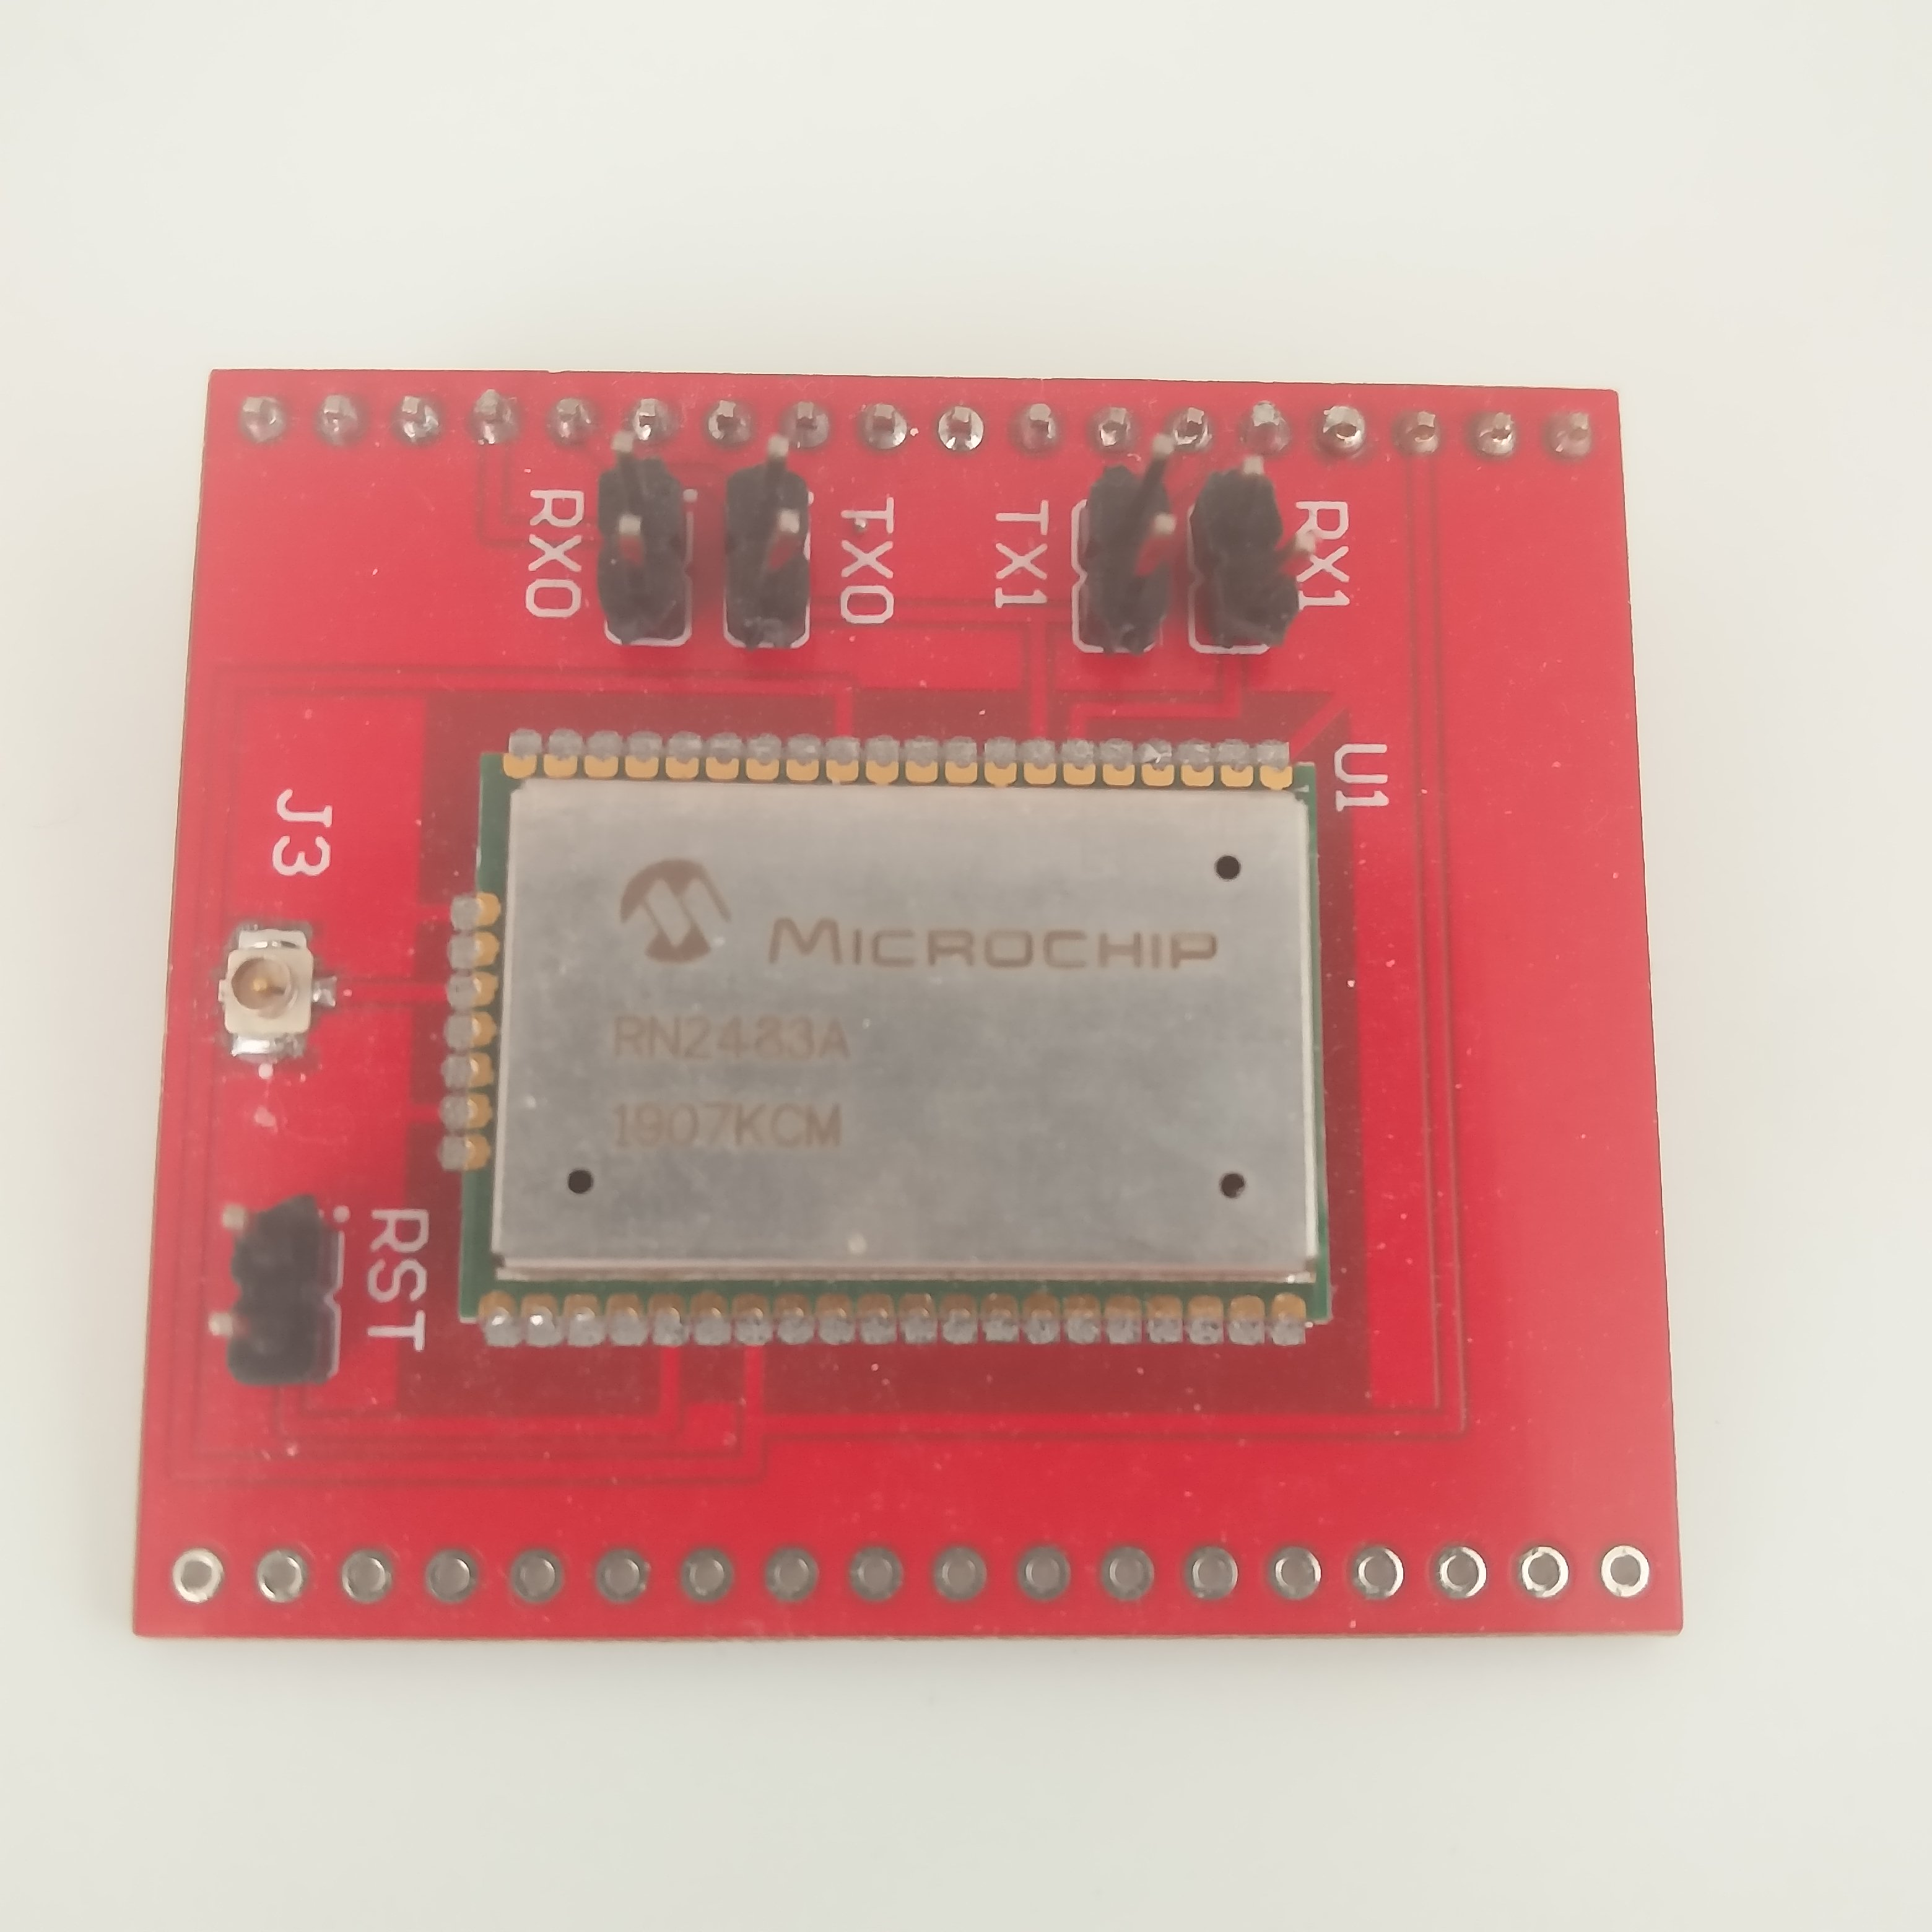
\includegraphics[width=0.6\textwidth]{thesis.tex/chapters/driver/fig/rn2483.jpg}
    \caption{The RN2483 LoRa radio shield\label{fig:rn2483pic}}
\end{subfigure}
\hfill
\begin{subfigure}[b]{.5\textwidth}
    \centering
    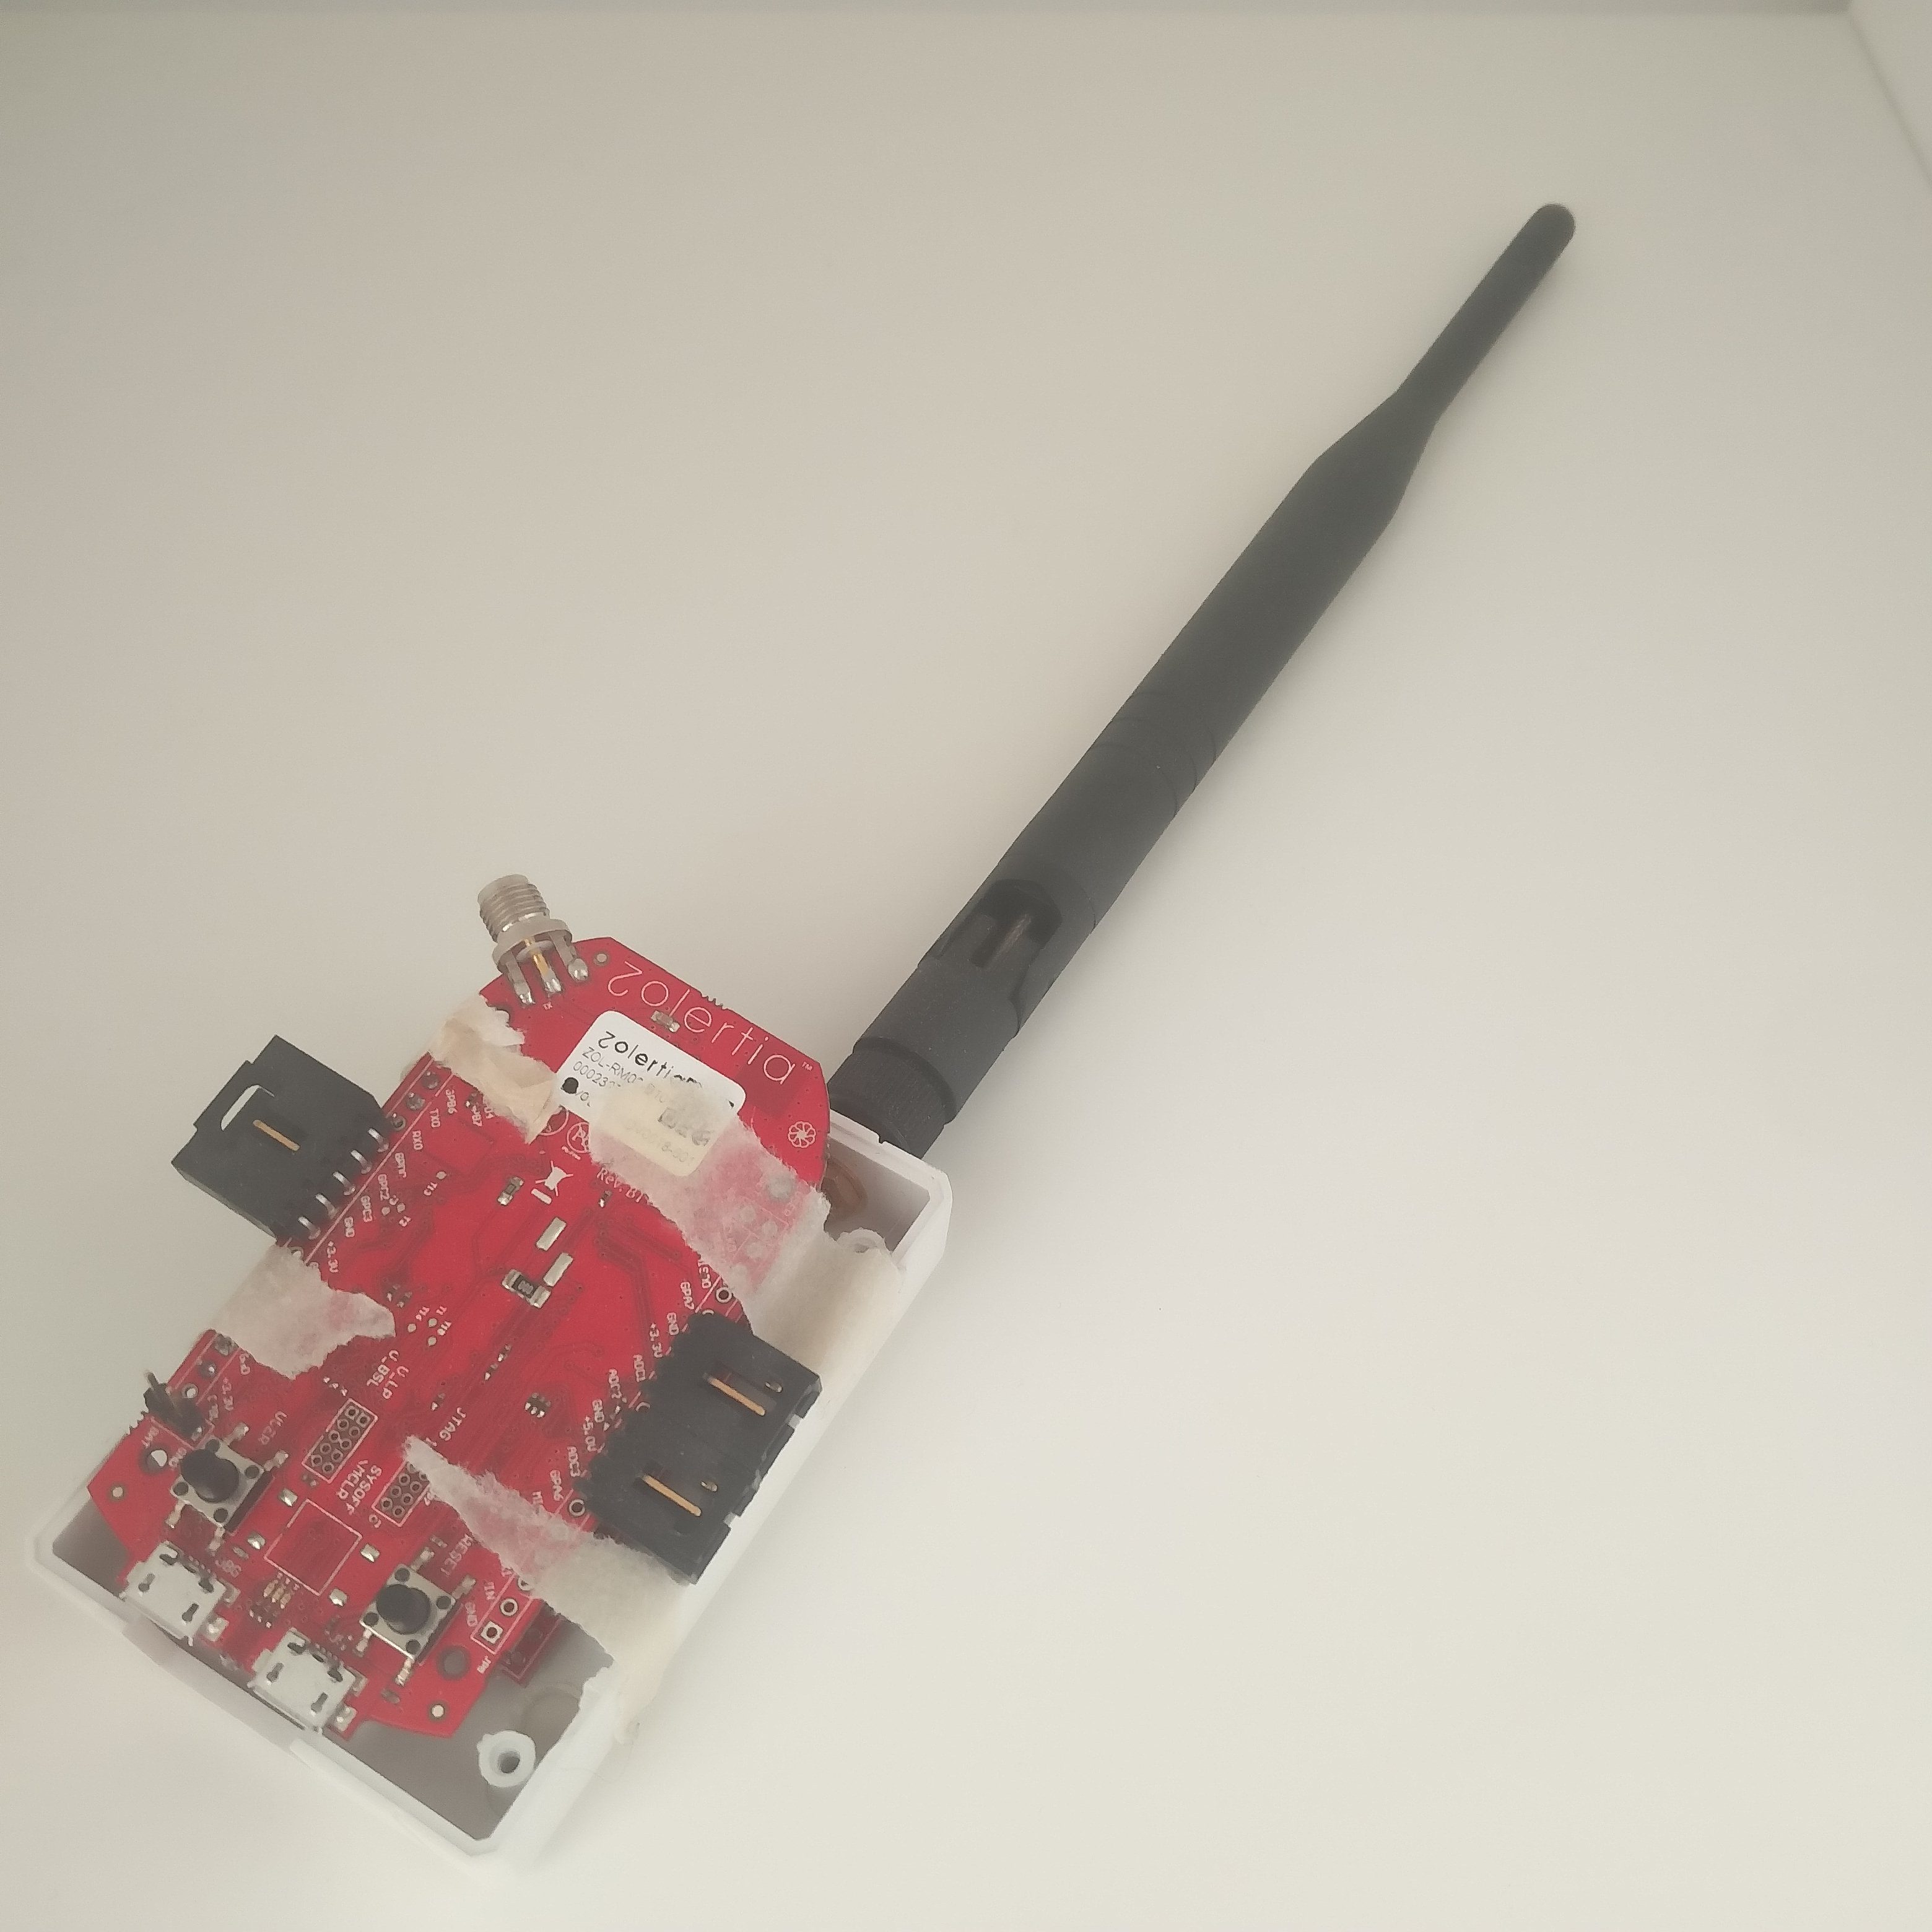
\includegraphics[width=0.6\textwidth]{thesis.tex/chapters/driver/fig/zolertia.jpg}
    \caption{The Zolertia RE-Mote with the shield\label{fig:zolpic}}
\end{subfigure}
\caption{The harware component I used\label{fig:hardused}}
\end{figure}

\section{RN2483 LoRa Radio Module Structure}

Developed by \emph{Microchip} the \emph{RN2483} is a LoRa radio module operating in
the 433 MHz and 868 MHz Frequency Bands~\cite{microchip:rn2483}.
The module is specifically designed to work with LoRaWAN compatible networks,
by including a set of commands designed for seamless integration with the
\emph{LoRaWAN Protocol Stack}

Each communication to and from the module is done via Universal asynchronous receiver-transmitter (UART) ASCII command,
making it easy for a human to interact with the module by typing commands
on a terminal and reading the response back in a readable format
(see~\ref{fig:pcconn}).
% The module is made for ease of use over performance and power consumption.

\begin{figure}[H] % TODO More info on axis
\centering
\begin{tikzpicture}[auto, thick]
  \node(pc) [server, label=below:{PC}] {};
  \node(ftdi) [draw, rectangle, right=of pc, right=4cm] {USB to UART Adapter};
  \node(module) [draw, rectangle, minimum size=6mm, right=of ftdi, right=2.5cm] (module) {RN2483 Module};

  \path (pc) edge[<->] node[]{USB Connection} (ftdi) ;
  \path (ftdi) edge[->,bend left] node[text width=1cm, align=center]{TX} (module);
  \path (module) edge[->,bend left] node[text width=1cm, align=center]{RX} (ftdi);
\end{tikzpicture}
\caption{Simple communication with the module scenario\label{fig:pcconn}}
\end{figure}


The module's interface includes three types of commands that enable access to
different functions~\cite{microchip:reference}.

\begin{itemize}
  \item \emph{radio} for the low-level radio commands to access the transceiver
    and PHY settings directly without the LoRaWAN interface overhead.
  \item \emph{mac} to access the LoRaWAN protocol stack configurations and
    commands. This command set will be used less because our implementation
    requires low-level transceiver access.
  \item \emph{sys} for the module-specific configurations such as the module
    GPIOs state, \emph{sleep}, EEPROM memory access, \ldots
\end{itemize}

\section{Contiki Radio Driver Implementation}

All the files for the driver implementation are available from
\href{https://github.com/tperale/contiki-ng}{github.com/tperale/contiki-ng}
in \lstinline{/arch/dev/rn2483} and
\lstinline{/examples/platform-specific/rn2483} folder.
The usage of each file is explained in Appendix~\ref{appendix:driver}.

\paragraph{}

The Contiki WIKI did not provide any information about writing our radio driver
or porting a new radio platform for Contiki.
Our implementation is based on the other radio driver implementation already
available on Contiki to understand the driver structure.

To create a Contiki radio driver we have to implement a \lstinline{radio_driver}
structure that must implement the following functions.

\begin{description}
  \item[init] is the first function of the driver executed at startup.
    The configuration of the RN2483 into point-to-point mode takes place here.
  \item[prepare] is the function called before data transmission.
    We can not transmit radio messages while listening for incoming messages, the
    first step of preparation is to exit the radio reception mode with the
    command \lstinline{radio rxstop}.
    The function takes care to convert the data in the command ready to be sent.
  \item[transmit] sends the already formatted command in the prepare function and
    waits for the \lstinline{radio_tx_ok} acknowledgement.
  \item[send] is the combination of \lstinline{prepare} and
    \lstinline{transmit}.
  \item[read], on radio message reception, the function copies the
    message to the buffer passed in the argument.
  \item[channel\_clear] verify there is no transmission ongoing on the channel.
  \item[receiving\_packet] should theoretically check if the radio module is
    currently getting a new message from a transmission. This is a function we
    can expect from some platforms with an integrated radio module but here the
    simplicity of the RN2483 shows its limitations and I found no way for the module
    to acknowledge when it receiving a new message.
  \item[pending\_packet] checks the message inbox to see if we received a new
    message.
  \item[on] wake-up the module and starts listening to radio messages.
  \item[off] stop listening to radio messages and put the module to sleep.
  \item[get\_value, set\_value, get\_object, set\_object] are all the functions used
    to configure the radio driver when manipulated by the upper layer.
    The parameters needed by TSCH will be discussed in Chapter~\ref{section:tsch}.
\end{description}

I will introduce the two main features of any radio driver, the transmit and receive
function, and how these functions work with the RN2483 radio module.
Before that, I will introduce the single design challenge of implementing a radio
driver based on UART communication on Contiki.

\subsection{Synchronous communication with the module}

The design challenge for the radio driver implementation is the
UART message mechanism implementation.
UART communication needs synchronous messaging for every
transmission, configuration, and reception.
Acknowledgements from commands avoid
clashes when trying to use the module at the same time.
The previous implementation in~\cite{8847137} used fixed time delays to
wait for the command to full execution on the module. This method
quickly showed its limitation, each command has its delay, and
fixed delays slow the global execution.

The Contiki UART driver for the processor I used (the CC2538) does not have synchronous
blocking read function out of the box, it assumes the programmer will compute the
responses from UART in processes waiting for an event instead.
Reception works by executing an \emph{input handler} at each interruption
triggered from UART reception.
Contiki set the default input handler with the function
\lstinline{serial_line_input_byte},
specifically designed for serial communication with terminals.
The function \lstinline{serial_line_input_byte} pass each character to standalone
process (\lstinline{serial_line_process}) and broadcast an event on command
full reception.
The drawback of Contiki design is the lack of a mechanism that allows programmers
to wait for an event inside a function.
Because driver implementation in Contiki requires the definition of function
I implemented a custom handler that directly treats each message in the
interrupt instead of using processes.
The custom handler is designed as a state machine (Fig~\ref{fig:cmdstate}) and
takes advantage of the limited response
format from the RN2483 radio module to sort each new communication.
When sending a command to the module the program will busy-wait for the
response. On response, an interrupt is triggered and the busy-waiting can stop.
If no response is received a timeout is triggered.

% \begin{itemize}
%   \item Asynchronous LoRa radio messages start with \lstinline{radio rx  }.
%   \item \lstinline{radio_tx_ok} indicates the end of the radio transmission.
%   \item \lstinline{ok} indicates the acknowledgement of a command.
% \end{itemize}

% I implemented helper functions, to ease the command transmission and
% acknowledgement between the RE-Mote and the RN2483.
%
% \begin{description}
%   \item[rn2483\_receive\_synch] busy-wait on the command states
%     (Fig~\ref{fig:cmdstate}) until reaching the \emph{received} state
%     or the timeout duration has elapsed.
%   \item[rn2483\_send\_cmd] a \emph{printf} style command, automatically
%     waiting for the acknowledgement (with the possibility to add custom timeouts).
%   \item[rn2483\_raw\_cmd] sending the command from a buffer in argument
%     without formatting or waiting for the acknowledgement.
% \end{description}

\begin{figure}[H]
\centering
  \begin{tikzpicture}[->,>=stealth',shorten >=1pt,auto,node distance=3.5cm]
  \tikzstyle{every state}=[thick,draw=gray!50,fill=gray!20,draw=none,text=black]

  \node[initial,state] (A)                    {Transmission};
  \node[state]         (B) [above right of=A] {Reception};
  \node[state]         (C) [below of=B]       {Timeout};
  \node[state]         (D) [right of=B]       {Received};

  \path (A) edge [bend right]    node {     } (B)
            edge [bend left]     node {     } (C)
        (B) edge [bend left]     node {     } (C)
            edge                 node {     } (D)
        (C) edge [bend left]     node {     } (A)
        (D) edge [bend right=85] node {     } (A);
\end{tikzpicture}
\caption{The command states\label{fig:cmdstate}}
\end{figure}


\subsection{Transmit}

The radio transmission command has a different pattern from the other commands
of the module.
After the acknowledgement of the radio transmission command (\lstinline{radio tx ...}),
the module transmits a second message when the radio communication is done.
Figure~\ref{fig:txsequence} shows how the command sequence between the RN2483
and Contiki through the UART.

\begin{figure}[H]
\centering

\begin{sequencediagram}

\newthread{A}{RE-Mote}{}
\newinst[1]{B}{RN2483}{}
\newinst[3]{C}{Radio Band}{}
\begin{call}{A}{radio tx~\ldots}{B}{radio\_tx\_ok}
  \messdash{B}{ok}{A}
  
  \begin{sdblock}{Radio Transmission}{Transmition time calculated
    in~\ref{eq:tpacket}}
    \begin{call}[4]{B}{}{C}{}
    \end{call}
  \end{sdblock}
\end{call}

\end{sequencediagram}

  \caption{\lstinline{radio tx} command sequence diagram\label{fig:txsequence}}

\end{figure}



Microchip chose to represent the payload as string formatted hex number to
facilitate the manual writing of commands, making the message payload twice as
long as its original content.
The driver function has to take care of translating the \emph{8-bit} number
array it receives to the hex number string representation.

\subsection{Receive}

The reception also follows a different scheme from the other commands.
New message reception can happen at any time, asynchronously, from the moment
we run the command \lstinline{radio rx 0}.
Because in TSCH, only one message can get received during a time slot
I implemented a one message inbox as we can see in Fig~\ref{fig:rxstate},
on new message the state is set in \emph{received} which notify the presence
of a message until its read.

Every message coming from the module is analyzed.
The radio communication that starts with \lstinline{radio rx }, set a flag to
indicate the presence of a new message, and thus switching to the \emph{received}
state.
This flag remains until the message is read from the driver with the
\lstinline{read} function where the state fallback into \emph{empty} state.
Messages are received in a string formatted hex number and are converted to an
\emph{8-bit integer array}.
Also, a timestamp is saved at the reception to keep track of when the
message was received.

\begin{figure}[H]
\centering
  \begin{tikzpicture}[->,>=stealth',shorten >=1pt,auto,node distance=3.5cm]
  \tikzstyle{every state}=[thick,draw=gray!50,fill=gray!20,draw=none,text=black]

  \node[initial,state] (A)              {None};
  \node[state]         (B) [right of=A] {Received};

    \path (A) edge [bend right] node[below] {Reception} (B)
          (B) edge [bend right] node[above] {Read} (A);
\end{tikzpicture}
\caption{The RX states\label{fig:rxstate}}
\end{figure}


\subsection{Device Configuration}

The module can be configured through the following structure.
It allows programmers to access LoRa different parameters from the code without
having to interact with the module.

\begin{lstlisting}[language=C]
typedef struct {
  radio_modulating_mode mod;
  radio_channel chan;
  uint32_t freq;
  radio_sf sf;
  radio_bw bw;
  radio_cr cr;
  uint32_t prlen;
  radio_pwr pwr;
  bool crc;
  bool iqi;
  bool explicit_header;
  uint32_t wdt;
} lora_radio_t;
\end{lstlisting}

This structure has a default definition but can be redefined from anywhere
by redefining \lstinline{RN2483_DEV_CONF}.
The currently used parameters are accessed with \lstinline{RN2483_DEV}.

We will see in Chapter~\ref{section:tsch} how those variables are used in
calculations.

\section{Validation}

To verify the implementation of the radio driver I made
a \emph{ping-pong} example based on the nullnet example already
available in \emph{contiki-ng}.
My example is located in \lstinline{/example/platform-specific/lora/nullnet}
and demonstrate the driver is correctly working with the upper layers of the
network stack.

I also implemented a shell to interact with the module that is described
in Appendix~\ref{appendix:shell}.

\subsection{Testing Setup}

My testing setup was the same as~\cite{8847137}. I used the Zolertia RE-Mote
Rev-B platform, using the CC2538 microcontroller, connected to the
RN2483 breakout board, as schematized in Fig~\ref{fig:schemaconn}.

The RE-Mote platform has two UART peripheral, the UART1 peripheral is used
to communicate with the module because the platform debugger uses UART0.

The \lstinline{PD0} GPIO is wired to the reset pin to allow
a software reset of the module as well as a push-button in case of hard reset.

\begin{figure}[H]
  \centering
  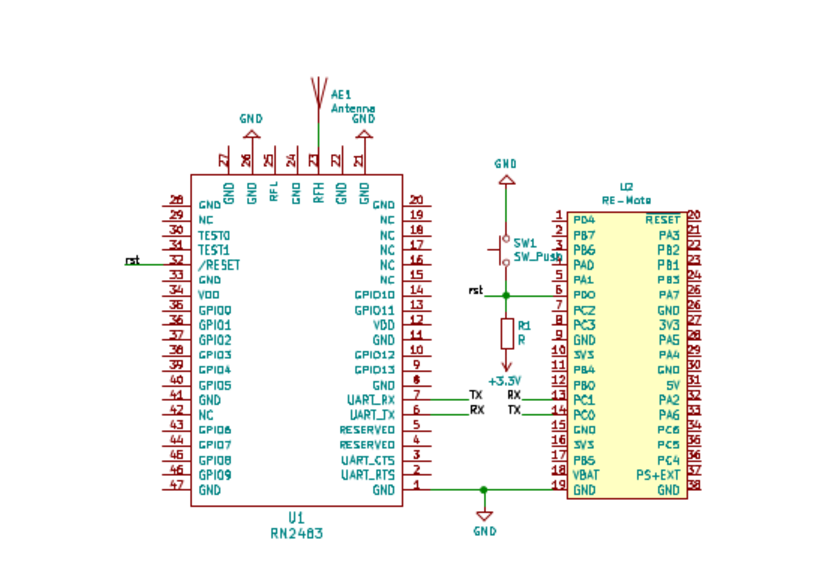
\includegraphics[scale=0.70]{thesis.tex/chapters/driver/fig/conn_diag.pdf}
  \caption{Hardware connection\label{fig:schemaconn}}
\end{figure}

\subsection{Ping-Pong\label{section:pingpong}}

This example is based on the \emph{nullnet-broadcast} example to test if two
nodes could communicate using the LoRa driver I implemented when controlled by
the \emph{CSMA} MAC layer instead of directly using the driver Application Programming Interface (API)\@.
Using a test with a simpler MAC protocol than TSCH, that do not need adaptation,
is the first test done to ensure my driver is correctly working before starting to adapt
the TSCH protocol.
The MAC protocol used is carrier Sense Multiple Access (CSMA).
The example is using the NETSTACK in Fig~\ref{fig:pingpongstack}.

\begin{figure}[H]
\centering
  \begin{tikzpicture}[->,>=stealth',shorten >=1pt,auto,node distance=1.6cm]

  \tikzstyle{comment}=[
    right=2pt,
    font=\small,
    fill=white,
    text=black,
    draw=black,
  ]

  \tikzstyle{every state}=[rectangle,thick,
    draw=black,fill=gray!20,text=black,
    minimum width= 6cm,
    minimum height= 1.20cm
  ]

  \tikzstyle{smallstate}=[rectangle,thick,
    draw=black,fill=gray!10,text=black,
    minimum width= 4cm,
    minimum height= 1.20cm
  ]

  \node[smallstate]         (A)                    {Null Net};
  \node[smallstate]         (B) [below of=A]       {Null Routing};
\begin{scope}[on background layer]
  \node[state, fit=(A)(B)] (AB)                 {};
\end{scope}
  \node[state,below=1cm]         (C) [below of=AB]       {CSMA};
  \node[state]         (D) [below of=C]       {LoRa};

  \node[comment]       at (AB.north west) {Network Layer};
  \node[comment]       at (C.north west) {MAC Layer};
  \node[comment]       at (D.north west) {Physical Layer};
  % \path (A) edge [bend right]    node {     } (B)
  %           edge [bend left]     node {     } (C)
  %       (B) edge [bend left]     node {     } (C)
  %           edge                 node {     } (D)
  %       (C) edge [bend left]     node {     } (A)
  %       (D) edge [bend right=85] node {     } (A);
\end{tikzpicture}
\caption{The network stack used for the ping-pong example\label{fig:pingpongstack}}
\end{figure}


The example is a simple two-way communication between two motes.
The first one is sending a request with a number as
payload and wait for the acknowledgement from the second motes sending back
the same payload.
No other request is sent until the acknowledgement is received.
This is schematized in Fig~\ref{fig:pingpongsequence}.

\begin{figure}[H]
\centering

\begin{sequencediagram}

\newthread{A}{Mote A}{}
\newinst[1]{B}{Mote B}{}

\begin{call}[4]{A}{ping}{B}{pong}
\end{call}
\end{sequencediagram}

\caption{Description of the execution of the ping-pong example\label{fig:pingpongsequence}}

\end{figure}



Running the example shows the LoRa driver works with CSMA and confirms
it follows correctly the Contiki radio driver specification.

\section{Conclusion}

This chapter detailed the RN2483 driver implementation I made for Contiki OS.
Designing and implementing a radio driver for a LoRa radio is the first step towards achieving LoRa
multi-hop network in Contiki.
We showed the steps to write a radio driver for the RN2483 in Contiki-NG and clarified how
the architecture of the module integrates with the driver architecture of Contiki-NG.
I explained how I overcome the design issues related to Contiki to achieve
synchronized UART communication.
Finally, to demonstrate the proper functioning of my driver I used a simple "ping-pong" example
using the CSMA MAC protocol, which is simpler protocol than TSCH.
This simple protocol enabled to handle my
driver and allowed to show that my design and implementation had correctly followed the Contiki driver
specification.

\paragraph{}

This chapter and the implementation content could be the basis of a future
driver implementation that would also require the use of UART.
This driver will be used in the next chapter where it will be directly
manipulated by the TSCH code.
